\section{Boomerang Design} \label{sec:design}

As previously discussed, the Boomerang protocol enhancement for Bitcoin is motivated by the need to hide the source from which transactions are introduced into the network. Furthermore, this should be done in a transparent way so that any other form of anonymous coin extension on top of Bitcoin (e.g., Zerocoin) can leverage the service for transaction anonymity. Boomerang is \emph{not} intended to support regular Bitcoin traffic; once a transaction becomes public knowledge, Boomerang no longer plays a role in its distribution. 

In the following sections we detail the core protocol and several important design and security tradeoffs that can be made in practice when using Boomerang. A formal analysis of the security and performance of Boomerang-enhanced Bitcoin is provided in Sections X and Y. 

\begin{table*}[ht!]
\begin{center}
\caption{Boomerang Protocol Notation}
	\begin{tabular}{|l|l|}\hline
	\textbf{Symbol} & \textbf{Description} \\ \hline
	$W$ & Local number of parallel circuits constructed to emit a new transaction. \\
	$D$ & Global depth of transaction and dummy message circuits. \\
	$T$ & A boomerang transaction \\ 
	$\bar{T}$ & An encrypted boomerang transaction \\ 
	$M$ & A (dummy or encoded transaction) Boomerang message sent over the wire. \\
	~ & A message is treated as an indexable array with fields shown in Figure \ref{fig:boomerang_message}. \\
	$\mathbf{C}$ & Set of valid nodes from which to build a circuit. \\
	$\mathsf{AV}$ & Address vector element of a Boomerang message. \\
	$\mathsf{addr}$ & Network address of a Bitcoin node. \\
	$E_{pk}(\cdot)$ & ECC-based encryption of some plaintext under the public key $pk$. \\	
	$D_{sk}(\cdot)$ & ECC-based decryption of some ciphertext under the private key $sk$. \\ \hline
	\end{tabular}
\end{center}
\end{table*}

\subsection{Boomerang Peer-to-Peer Network Design}
Boomerang peer discovery is done in a similar manner to the Bitcoin peer discovery process described above with a few exceptions. Boomerang nodes can also query Bitcoin nodes after connecting to the Bitcoin network. Boomerang nodes can also learn the address of other nodes by routing Boomerang messages. The Boomerang peer discovery methods are:

\begin{enumerate}
	\item User inputted addresses from command line or text file: If the user manually inputs address information, the client will attempt to connect to those Boomerang peers first.
	\item Node reads stored Boomerang addresses from previous sessions: Boomerang clients will attempt to connect to peers stored in the internal address database from the previous session.
	\item Nodes make a DNS request for Boomerang seed nodes: If there are no active nodes in the internal address database, then the client will perform a DNS lookup using hard-coded DNS servers for current seed nodes.
	\item Nodes connect to hard-coded seed addresses: If DNS lookups fail, then the client attempts to connect to hard-coded seed addresses.
	\item Nodes query Bitcoin network for Boomerang nodes: The client sends Boomerang connection requests to nodes on the Bitcoin network.
	\item Nodes utilize callback addresses: After receiving a Boomerang connection request from a remote node, the client node can use the callback address to connect to the remote node and exchange address database information.
	\item Nodes receive relayed addresses: After receiving new address information and verifying validity of the address, a node will randomly pick a few nodes in the internal database and relay the new address information.
	\item Nodes will self broadcast periodically: Similarly to relayed addresses, periodically Boomerang clients will randomly pick a few nodes in the internal database and relay its own address information.
	\item Boomerang messages: The destination of a Boomerang message must be a Boomerang node. The client can then request a connection with the destination node and exchange address database information.
\end{enumerate}

\subsection{Transaction Encode and Broadcast Protocol} \label{sec:broadcast-protocol}

At the heart of the Bitcoin protocol is the ability to encode new transactions as Boomerang messages and then ripple them throughout the network. We describe the complete procedure for message encoding, {\sf EncodeTransaction}, in Algorithm \ref{alg:encode}, where the notation contained therein is defined in Table \ref{tab:notation}. This procedure takes only two parameters - a transaction $T$ to encode and a set of valid nodes $\mathbf{C}$ to be used in the circuit(s) creation, where $\mathbf{C}$ is created by randomly sampling from the set of valid nodes in the address book (see Section \ref{sec:validation} for a description of how the address book is managed). An encoded Boomerang message has a very well-defined format, as shown in Figure \ref{fig:boomerang_message}, composed of seed element, encrypted address vector, encrypted message identifier (used internally during message validation), and the encrypted transaction. In particular, the message is composed of the following:
\begin{enumerate}
	\item A potentially re-encrypted seed. By the description of {\sf EncodeTransaction}, it is required that the public-key encryption scheme used to mask these seeds has the same domain and range. This is needed because the decrypted seed for one hop will be used as decrypted seed on the previous hop, very much like onion layers of encryption.
	\item An encrypted address vector that is used by each hop to learn the next hop in the circuit without learning any other information about the nodes in the circuit. More specifically, a router can only learn about the immediate source and destination of a Boomerang message (the security and anonymity implications of this are discussed in the following section).
	\item A potentially re-encrypted transaction message block. This block either stores the encrypted transcaction, where the encryption is done by XORing with a pseudorandom bit string generated by the decrypted seed value, or the plaintext transaction that is to be broadcast throughout the network.
\end{enumerate}

% \begin{figure}[ht!]
% \begin{center}
% 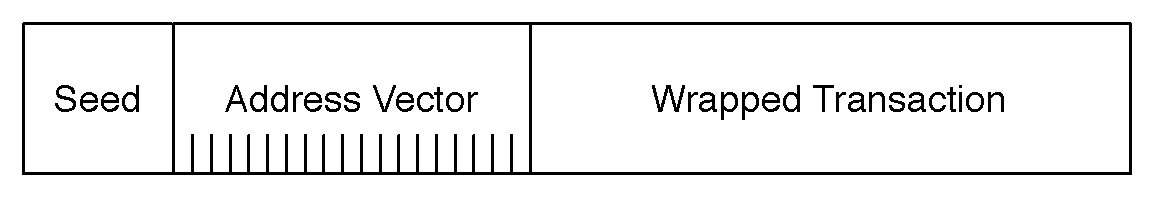
\includegraphics[scale=0.35]{./images/boomerang_message.pdf}
% \caption{Boomerang message encoding.}
% \label{fig:boomerang_message}
% \end{center}
% \end{figure}
\begin{table*}
\begin{center}
\caption{Boomerang encoded message format.}
\label{tab:msg-header}
    \begin{tabular}{|c|c|c|l|} \hline
    \textbf{Field Size (bits)} & {\bf Description} & {\bf Data Type} & {\bf Comments} \\ \hline
    $256$ & Seed scratch & uint8\_t[32] & This field is an element on the elliptic curve over the field $\mathbb{F}_p$. \\
    $512D$ & Encrypted address vector & uint8\_t[$D$][64] & Encryption of the address vector used to define the circuit trajectory. \\
    $*$ & Encoded transaction & uint8\_t[] & Encoded transaction field with width equal to the maximum encoded transaction size. \\ \hline
    \end{tabular}
\end{center}
\end{table*}

The procedure to handle Boomerang messages, {\sf BoomerangMessageHandler}, is provided in Algorithm \ref{alg:handler}. 

\begin{algorithm}[t!]
\caption{{\sf EncodeTransaction}($T, \mathbf{C}$)}
\label{alg:encode}
\begin{algorithmic}[1]

\For{$i = 1$ to $W$}
	\State $\bar{T} := T$
	\State $s \gets \{0,1\}^{\tau}$
	\For{$j = 1$ \textbf{to} $D_i$}
		\State $p := \mathsf{PRG}(s)$
		\State $\bar{T} := \bar{T} \oplus p$
		\State $s \gets E_{pk_{i,j}}(s)$
	\EndFor

	% populate the address vector
	\State $\mathsf{index} \gets \{0,\dots,2D_i\}$ % random address vector index
	\State $\mathsf{AV} := [2D_i]$ % address vector
	\For{$j = D_i$ \textbf{downto} $2$}
		\State $\mathsf{AV}[\mathsf{index}] := E_{pk_{i,j}}(\mathsf{addr}_{D_j})$
		\State $\mathsf{index} := \mathsf{index} + 1 (\mod N_m)$
		\State $\mathsf{AV}[\mathsf{index}] := E_{pk_{i,j}}(\mathsf{addr}_{D_{j-1}})$
		\State $\mathsf{index} := \gets \{0,\dots,2D_i\}$
		\While {$\mathsf{index} \mod 2 \not= 0$ \text{ and } $\mathsf{AV}[\mathsf{index}] \not= \bot \text{ and } \mathsf{AV}[\mathsf{index + 1 (\mod D_i)}] \not= \bot$}
			\State $\mathsf{index} \gets \{0,\dots,2D_i\}$
		\EndWhile
	\EndFor

	\State $M := \mathsf{Pack}(s, \mathsf{AV}, \bar{T})$
	\State $\mathsf{Transmit}(M)$
\EndFor

\end{algorithmic}
\end{algorithm}

\begin{algorithm}[t!]
\caption{{\sf BoomerangMessageHandler}($j$, $M$)}
\label{alg:handler}
\begin{algorithmic}[1]

\State $s := D_{sk_{j}}(M[0])$
\State $\bar{T} := M[2] \oplus PRG(s)$
\If {$\bar{T}$ is a well formed transaction}
	\State $\mathsf{Broadcast}(\bar{T})$ to the Bitcoin network
\ElsIf {$\bar{T}$ destination address is $\mathsf{addr}_j$}
	\State Discard $\bar{T}$; return;
\Else
	\State $\mathsf{AV} := M[1]$
	\State $i := 1$
	\While {$i < \mathsf{len}(\mathsf{AV})$}
		\State $\mathsf{addr}_{src} := D_{pk_j}(AV[j])$
		\If {$\mathsf{addr}_{src} = \mathsf{addr}_j$}
			\State $\mathsf{addr}_{dst} := D_{pk_j}(AV[j + 1])$
			\State $M := \mathsf{Pack}(s, \mathsf{AV}, \bar{T})$
			\If {$|Buffer| \geq B$}
				\State $\mathsf{Transmit}(M)$
			\Else
				\State $B.add(M)$
			\EndIf
		\Else
			\State $i := i + 2$
		\EndIf
	\EndWhile
\EndIf

\end{algorithmic}
\end{algorithm}

Similar to the Tarzan P2P mixnet, a critical part of the Boomerang protocol is the inclusion of cover traffic that is indistinguishable from legitimate encoded Boomerang transaction messages \cite{tarzan}. This traffic is needed for two reasons: (1) to keep legitimate transactions moving through mixnet circuits, and (2) to obfuscate the flow of legitimate transactions through the network. To support this cover traffic with minimal changes to the protocol, nodes in the network will \emph{reuse} and \emph{re-encode} old transactions to be sent throughout the network, with the exception that the destination node for the mixnet circuit (as specified in the {\sf EncodeTransaction} procedure) will be the same as the sender. This is because the sender can easily discover when a transaction message has looped through the network and back to themselves, at which point they can then simply discard the transaction. Clearly, the rate at which this cover traffic is generated plays a critical role in the overall performance of the system when using Boomerang. We discuss the selection of parameters that achieve optimal performance without sacrificing security in Section 5. 

\subsection{Peer Discovery Messages}
There are two types of Boomerang messages: peer discovery and maintenance messages, and encoded transaction and dummy messages. The encoded transaction and dummy messages were already described in Section \ref{sec:broadcast-protocol}. Here, we describe the format of the following peer discovery and maintenance messages: {\tt Version}, {\tt VerAck}, {\tt GetAddr}, and {\tt Addr}. Every one of such messages is prepended with a standard header whose format is shown in Table \ref{tab:msg-header}. The {\tt Version} message is used to establish a connection with a remote node, relay address information about a remote node, and verify Bitcoin protocol compatibility. Version messages are composed of the standard message header and the fields listed in Table \ref{tab:msg-version}. In response to a {\tt Version} message, {\tt VerAck} messages are sent from the recipient to the original sender. These messages include the standard message header and the fields listed in Table \ref{tab:msg-verack}. The {\tt GetAddr} messages are composed of just the standard header - the body of the message is empty. Intuitively, one may think of these as short messages broadcasted throughout the group. Finally, the {\tt Addr} message contains information about active nodes on the network. An active node is a node that has been validated within the last 3 hours (this time parameter may differ on a per-client basis). The {\tt Addr} message contains the standard message header and the fields listed in Table \ref{tab:msg-addr}. 

\begin{table*}
\begin{center}
\caption{Message header format.}
\label{tab:msg-header}
    \begin{tabular}{|c|c|c|l|} \hline
    \textbf{Field Size} & {\bf Description} & {\bf Data Type} & {\bf Comments} \\ \hline
    4 & magic & uint32\_t & Magic value indicating message origin network, and used \\
    ~ & ~ & ~ & to seek to next message when stream state is unknown \\
    12 & command & uint8\_t[12] & ~ \\
    4 & length & uint32\_t & Length of payload in number of bytes \\
    4 & checksum & uint32\_t & First 4 bytes of SHA256(SHA256(payload)) \\ \hline
    \end{tabular}
\end{center}
\end{table*}

\begin{table*}[ht!]
\begin{center}
\caption{{\tt Version} message format.}
\label{tab:msg-version}
    \begin{tabular}{|c|c|c|l|} \hline
    \textbf{Field Size} & {\bf Description} & {\bf Data Type} & {\bf Comments} \\ \hline
    4 & version & int32\_t & Identifies protocol version being used by the node \\
    8 & services & uint64\_t & bitfield of features to be enabled for this connection \\
    8 & timestamp & int64\_t & standard UNIX timestamp in seconds \\
    26 & addr\_recv & net\_addr & The network address of the node receiving this message \\
    26 & addr\_from & net\_addr & The network address of the node emitting this message \\
    8 & nonce & uint64\_t & Node random nonce, randomly generated every time a version packet is sent. \\
    ~ & ~ & ~ & This nonce is used to detect connections to self.
 \\
    ? & user\_agent & var\_str & User Agent (0x00 if string is 0 bytes long) \\
    4 & coin\_version & int32\_t & Identifies Bitcoin protocol version being used \\
    4 & start\_height & int32\_t & The last block received by the emitting node \\
    32 & hash public key & uint8\_t[32] & Hash of public key used by the node \\ \hline
    \end{tabular}
\end{center}
\end{table*}

\begin{table*}[ht!]
\begin{center}
\caption{{\tt VerAck} message format.}
\label{tab:msg-verack}
    \begin{tabular}{|c|c|c|l|} \hline
    \textbf{Field Size} & {\bf Description} & {\bf Data Type} & {\bf Comments} \\ \hline
    256 & public key & uint8\_t[32] & Public key used by the recipient node \\ \hline
    \end{tabular}
\end{center}
\end{table*}

\begin{table*}[ht!]
\begin{center}
\caption{{\tt Addr} message format.}
\label{tab:msg-addr}
    \begin{tabular}{|c|c|c|l|} \hline
    \textbf{Field Size} & {\bf Description} & {\bf Data Type} & {\bf Comments} \\ \hline
    1+ & count & var\_int & Number of address entries (max: 1000) \\
    30x? & addr\_list & (uint32\_t + uint8\_t[32] + net\_addr)[] & Address of other nodes on the network. Each address \\
    ~ & ~ & ~ & also includes timestamp of the last time the node was seen \\
    ~ & ~ & ~ & active as well as the hash of the public key the node uses. \\ \hline
    \end{tabular} 
\end{center}
\end{table*}

\subsection{Node Connections}
To connect to a remote node, the client sends a version message, which contains Bitcoin network information, Boomerang version, and a hash of the client’s public key. If the remote node accepts the information in the version message, it will reply with a verack message that contains the remote node’s public key as well as its own version message.  The client will reply with a verack message, which contains the client public key, if it accepts both messages from the remote node.  Both nodes then add the address, public key, and time in their respective internal databases.

\subsection{Node Validation}
Boomerang clients draw from a pool of validated addresses for sending Boomerang transactions. If this pool is less than 1,000, Boomerang will begin to use dummy Boomerang messages to validate new addresses. The pool of addresses to be validated is equal to the number of validated addresses needed to reach the 1,000 address cap and is comprised of the most recently active non-validated addresses. If the pool of addresses is too small, Boomerang will begin sending getaddr queries to increase the pool size. An address is considered non-validated if it either has an invalid validation timestamp or a timestamp older than 3 hours. When a remote node’s address is added to the pool of addresses to be validated, the client must check if it has the node’s public key. If the address was added from a relayed addr message, the client must connect to the remote node in order to obtain the public key. If the connection could not be made, then the address is removed from the internal database and pool.

In order to validate addresses, dummy Boomerang messages will be routed through the addresses chosen from the pool of “addresses to be validated” as well as validated addresses. If the Boomerang message returns to the client and decrypts correctly, the nodes along the message’s route are marked as verified with a second timestamp in the internal database. Both first timestamp, which keeps track of when the node was last seen as active, and the second validation timestamp are updated with the time the message arrived plus a small random number (from 0 to an hour). Boomerang will also update the timestamps if a transaction message sent by the client is heard over the Bitcoin network. Boomerang clients will only relay address information from addresses verified in the last 3 hours and never reveal the validation timestamp.

\subsection{Cryptographic Primitives}

Based on the {\sf EncodeTransaction} and {\sf BoomerangMessageHandler} procedures, we require the following cryptographic primitives to support Boomerang messages:
\begin{enumerate}
	\item Efficient chosen plaintext secure (CPA-secure) public-key encryption \footnote{The observant reader may see that CCA-security would be better suited for this design since it more accurately models a real-world adversary who can maliciously send malformed Boomerang messages with chosen ciphertexts to an honest node and observe the decrypted seed value that is output. However, since nodes will accumulate messages prior to mixing, an adversary cannot be sure \emph{which} output message corresponded to their input message, and therefore the likelihood of an adversary discovering the plaintext associated with their chosen ciphertext is small.} with regards to computational complexity and bandwidth requirements. 
	\item Deterministic PRG whose input is an element in the range specified by the public-key encryption scheme.
\end{enumerate}

To satisfy the first primitive for public-key encryption and decryption, Boomerang leverages standard public-key elliptic curve cryptosystem over the NIST-recommended field $\mathbb{F}_{p}$, where $|p| = 256$ (the size of prime $p$ in bits) \cite{nist-curves}. The domain parameters for the Boomerang encryption scheme are specified below:
\begin{itemize}
	\item $p$ - the prime number defining the finite field over which all elliptic curve operations are performed.
	\item $a, b$ - the coefficients that define the elliptic curve - $y^2 = x^3 +ax + b \mod p$.
	\item $G$ - the generator base point for the field.
	\item $n$ - the order of the curve generator point $G$ (i.e., the number of points on the field).
	\item $h$ - the cofactor of the field (unused for encryption and decryption).
\end{itemize}
For completeness, we provide a brief (and modified) description of the setup, key generation, encryption, and decryption procedures used by the cryptosystem, denoted {\sf Setup}, {\sf KeyGen}, {\sf Enc}, and {\sf Dec}, respectively, as used in Boomerang. 
\begin{itemize}
	\item {\sf Setup}: Generate and output domain parameters $p,a,b,G,n$ and $h$. 
	\item {\sf KeyGen}: Select a random integer $sk$ such that $0 < sk < n$ and compute $pk = sk \cdot G$. Output the public and private key pair $(pk, sk)$.
	\item {\sf Enc}($pk, m$): Select a random integer $r$ such that $0 < r < n$, compute $R = r \cdot G$, $S = r \cdot pk$ ($S$ is the ``secret'' mask), $T = m \oplus \mathsf{DPRG}(S)$. Output the ciphertext tuple $(R, T)$.
	\item {\sf Dec}$(sk, (R, T))$: Compute $S = sk \cdot R = sk \cdot r \cdot G = r \cdot (sk \cdot G) = r \cdot pk$, $m = T \oplus \mathsf{DPRG}(S)$.
\end{itemize}
Traditionally, the element $S$ is used to generate a symmetric key used to encrypt some message $m$. In our modified scheme, the element $S$ \emph{is used to generate a one-time pad} of the message $m$ using a deterministic pseudorandom bit generator (DPRG), and $R$ is used to recover the seed to remove this pad. Since $r$ is chosen uniformly at random, the seed to the DPRG is uniformly random, and by definition the encryption $m \oplus DPRG(S)$ is CPA-secure. 

To satisfy the second primitive for the PRG, Boomerang leverages the counter mode deterministic pseudorandom bit generator (CTR-DRBG) algorithm as specified in \cite{nist-prng} with AES-128 security strength (there is no security reason why this is chosen over Hash-DRBG or HMAC-DRBG). The CTR-DRBG takes as input a $256$-bit seed to achieve AES-128 security (a seed derivation function could be used, but we omit this from the design). To use CTR-DRBG, a node must instantiate the state of the algorithm by specifying an entropy input, personalization string (fixed), and security strength parameter (optional, but assumed to be AES-128). To pump out pseudorandom bits, the update procedure is invoked using the state of the algorithm and the specified seed, as shown in Figure \ref{fig:ctr_drbg_update}, to produce the required number of output bits $V$ (note that the internal state value for $Key$ is populated when the algorithm is instantiated). 

\begin{figure}[ht!]
\begin{center}
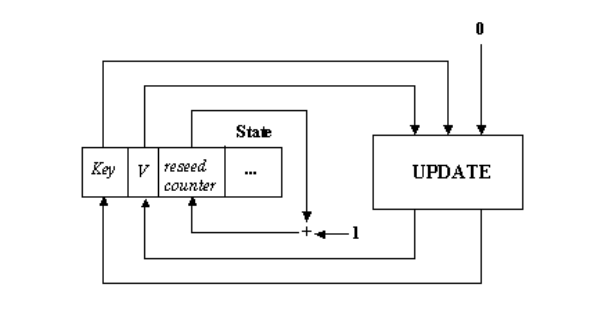
\includegraphics[scale=0.35]{./images/ctr_drbg_update.png}
\caption{CTR-DRBG update procedure.}
\label{fig:boomerang_message}
\end{center}
\end{figure}

\subsection{Boomerang Congestion Control}
An obvious downside of the Boomerang design is that improper parameter selection (i.e., cover traffic generation rates, lengthy circuits, etc) can lead to network congestion and self-induced denial of service attacks. To this end, we propose the following congestion control strategy, motivated by the window-based congestion control algorithm in TCP Reno. Each node will maintain a window 

